\RequirePackage[l2tabu, orthodox]{nag}%TODO: Remove this line after checking
%\documentclass[11pt, a4paper,twoside]{scrartcl} % Seminar
\documentclass[technote,a4paper,leqno]{IEEEtran}
\pdfoutput=1

% packages
\usepackage[utf8]{inputenc}
\usepackage[T1]{fontenc}
\usepackage{tabularx}
\usepackage{amsmath,amssymb}
\usepackage[pdftex]{graphicx}
\usepackage{caption}
\usepackage[hang]{subfigure}
\captionsetup{format=hang}
\usepackage{url}
\usepackage{ifthen}
\usepackage{url}
\usepackage{breakurl}
\usepackage[super]{nth}
\usepackage[breaklinks]{hyperref}
\def\UrlBreaks{\do\/\do-}
\usepackage[absolute,overlay]{textpos}
\usepackage{tikz}
\usepackage{csquotes}
\usepackage{booktabs}  % for \toprule, \midrule and \bottomrule
\usepackage{pbox}
\usepackage{braket} % needed for nice printing of sets
\usepackage[english]{babel}
\usepackage[headsepline,footsepline,plainheadsepline]{scrpage2}
\usepackage{changepage}
\usepackage{mathtools}
\usepackage[inner=3cm,outer=2.5cm,top=2.5cm,bottom=2cm,includeheadfoot]{geometry}
\usepackage[xindy,toc]{glossaries}
\loadglsentries[main]{glossary}
\makeglossaries

% Packages like in our pixel-wise-street-segmentation
% nameinlink, noabbrev: not supported by arxiv :-(
\usepackage[nameinlink, noabbrev,capitalise]{cleveref} % has to be after hyperref, nthe l.137 ...eam attr{/N 4}  file{sRGBIEC1966-2.1.icmorem, amsthm


% List stuff
\usepackage{enumitem}
\crefname{problemnr}{\textup{problem}}{\textup{problems}}
\newlist{problemnr}{enumerate}{1}
\setlist[problemnr]{label={P\arabic*}, ref=P\arabic*}
\crefalias{problemnri}{problemnr}


\usepackage[binary-units,group-separator={,}]{siunitx}
\sisetup{per-mode=fraction,
         binary-units=true,
         group-separator = {\,},
         range-phrase=-}
\DeclareSIUnit\pixel{px}
\usepackage{microtype}

\DeclareGraphicsExtensions{.jpg}
\DeclareMathOperator{\sgn}{sgn}
\DeclareMathOperator*{\minimize}{minimize}
\DeclareMathOperator*{\maximize}{maximize}

\newcommand\independent{\protect\mathpalette{\protect\independenT}{\perp}}
\def\independenT#1#2{\mathrel{\rlap{$#1#2$}\mkern2mu{#1#2}}}

\newcommand{\titleboth}{The State of the Art in Image Segmentation} %TODO: Really?
\title{\titleboth}
\author{Martin Thoma\\% ORCID: http://orcid.org/0000-0002-6517-1690 Thoma, Martin
info@martin-thoma.de
}

% arxiv doesn't like \sep
\hypersetup{
    pdfauthor   = {Martin Thoma},
    pdfkeywords = {semantic segmentation, pixelwise classification, pixel-level classification},
    pdfsubject  = {Segmentation},
    pdftitle    = {\titleboth},
}

\begin{document}
\maketitle
%!TEX root = vorlage.tex

\begin{abstract}
This survey gives an overview over different techniques used for pixel-level
semantic segmentation. It is based on an extensive literature review. Metrics
and datasets for the evaluation of segmentation algorithms, traditional
approaches for segmentation as well as recently published approaches with
convolutional neural networks and typical problematic situations for segmentation
algorithms are examined.
\end{abstract}


%!TEX root = vorlage.tex

\section{Introduction}\label{sec:introduction}
Semantic segmentation is the task of clustering parts of images together which
belong to the same object class. This type of algorithm has several use-cases
such as detecting road signs~\cite{4220659}, detecting tumors in
medicine~\cite{moon2002automatic}, detecting medical instruments in
operations~\cite{wei1997automatic}, colon crypts
segmentation~\cite{cohen2015memory}, land use and land cover
classification~\cite{huang2002assessment}. In contrast, non-semantic
segmentation only clusters pixels together based on general characteristics of
single objects. Hence the task of non-semantic segmentation is not
well-defined, as many different segmentations might be acceptable.

Several applications of segmentation are listed
in~\cite{annurev.bioeng.2.1.315}.

Object detection, in comparison to semantic segmentation, has to distinguish
different instances of the same object. While having a semantic segmentation is
certainly a big advantage when trying to get object instances, there are a
couple of problems: neighboring pixels of the same class might belong to
different object instances and regions which are not connected my belong to the
same object instance. For example, a tree in front of a car which visually
divides the car into two parts.

This paper is organized as follows: It begins by giving a taxonomy of
segmentation algorithms in \cref{sec:taxonomy}. A summary of quality measures
and datasets which are used for semantic segmentation follows in
\cref{sec:evaluation-and-datasets}. A summary of the most important traditional
segmentation algorithm and their characteristics follows in
\cref{sec:traditional-approaches}, as well as a very brief, non-exaustive
summary of recently published semantic segmentation algorithms which are based
on neural networks in \cref{sec:nn}. Finally, \cref{sec:problems} informs the
reader about typical problematic cases for segmentation algorithms.

% TODO: As speed is one of the hard requirements in practical applications, we
% outline some of the actions that can be applied to improve the speed of
% segmentation algorithms. Finally, I mention some of the publications which
% examine automatic image enhancement.

%!TEX root = vorlage.tex
% Martin Thoma

\section{Taxonomy of Segmentation Algorithms}\label{sec:taxonomy}
The computer vision community has published a wide range of segmentation
algorithms so far. Those algorithms can be grouped by the kind of data they
operate on and the kind of segmentation they are able to produce.

The following subsections will give four different criteria by which
segmentation algorithms can be classified.

This survey describes fixed-class (see \cref{subsec:allowed-classes}),
single-class affiliation (see \cref{subsec:class-affiliation}) algorithms which
work on grayscale or colored single pixel images (see \cref{subsec:input-data})
in a completely automated, passive fashion (see \cref{subsec:operation-state}).

\subsection{Allowed classes}\label{subsec:allowed-classes}
Are the classes which are to be distinguished known at the time when the
algorithm is developed or trained, or might there occur several objects which
were never seen before?

Most algorithms work with a fixed set of classes; some even only work on binary
classes like \textit{foreground vs background}~\cite{4228537} or \textit{street
vs no street}~\cite{bittel2015pixel}.

There are also unsupervised segmentation algorithms which do not distinguish
classes at all (see \cref{subsec:unsupervised-traditional-segmentation}) as
well as segmentation algorithms which are able to recognize when they don't
know a class. For example, in~\cite{gould2008multi} a
\textit{void class} was added for classes which were not in the training set.


\subsection{Class affiliation of pixels}\label{subsec:class-affiliation}
Humans do an incredible job when looking at the world. For example, when we
see a glass of water standing on a table we can automatically say that there is
the glass and behind it the table, even if we only had a single image and were
not allowed to move. This means we assign the coordinates of the glass at the
same time two labels: Glass and table. Although there is much more work being
done on \textit{single class affiliation} segmentation algorithms, there is a
publication about \textit{multiple class affiliation}
segmentation~\cite{levin2008spectral}. Similarly, recent publications in
pixel-level object segmentation used layered models~\cite{yang2012layered}.


\subsection{Input Data}\label{subsec:input-data}
The available data which can be used for the inference of a segmentation varies
by application.

\begin{itemize}
    \item \textbf{Grayscale vs colored}: Grayscale images are commonly used in
          medical imaging such as \gls{MR} imaging or ultrasonography whereas
          colored photographs are obviously widespread.
    \item \textbf{Excluding or including depth data}: RGB-D, sometimes also
          called range~\cite{hoover1996experimental} is available in robotics,
          autonomous cars and recently also in consumer electronics such as
          Microsoft Kinect~\cite{6190806}.
    \item \textbf{Single image vs stereo images vs co-segmentation}: Single
          image segmentation is the most wide-spread kind of segmentation, but
          using stereo images was already tried in~\cite{boykov2001fast}. It
          can be seen as a more natural way of segmentation as most mammals
          have two eyes.
          Co-segmentation as in~\cite{1640859,collins2012random} is the problem
          of finding a consistent segmentation for multiple images. This problem
          can be seen in two ways: One the one hand, it can be seen as the problem
          of finding common objects in at least two images. On the other hand,
          every image after the first can be used as an additional source of
          information to find a meaningful segmentation. This idea can be
          extended to time series such as videos.
    \item \textbf{2D vs 3D}: Segmenting images is a 2D~segmentation task where
          the smallest unit is called a \textit{pixel}. In 3D data, such as
          volumetric X-ray CT images as they were used in~\cite{929615}, the
          smallest unit is called a voxel.
\end{itemize}


\subsection{Operation state}\label{subsec:operation-state}
The operation state of the classifying machine can either be \textit{active} as
in~\cite{schiebener2011segmentation,schiebener2012discovery} where robots can
move objects to find a segmentation or \textit{passive}, where the received
image cannot be influenced. However, being in a passive situation can be
divided further by separating segmentation algorithms working in a completely
\textit{automatic} fashion versus algorithms working in an \textit{interactive}
mode. One example would a system where the user clicks on the background or
marks a coarse segmentation and the algorithm finds a fine-grained
segmentation.
\cite{boykov2000interactive,rother2004grabcut,protiere2007interactive}~describe
systems which work in an interactive mode.

%!TEX root = vorlage.tex

\section{Evaluation and Datasets}\label{sec:evaluation-and-datasets}

%!TEX root = vorlage.tex

\subsection{Quality measures for evaluation}%
\label{subsec:quality-measures}%
A performance measure is a crucial part of any machine learning system, but
there are other measures of quality which matter when segmentation algorithms
are compared. This section gives an overview of those quality measures.


\subsubsection{Accuracy}
Showing the correctness of the segmentation hypotheses is done in most
publications about semantic segmentation. However, there are a couple of
different ways how this accuracy can be displayed. One way to give readers a
first impression of the obtained segmentations is by showing examples such
as~\cref{fig:segmentation-example}.

\begin{figure}
\centering
\subfigure[Example Scene]{
  \label{fig:segmentation-example-scene}
  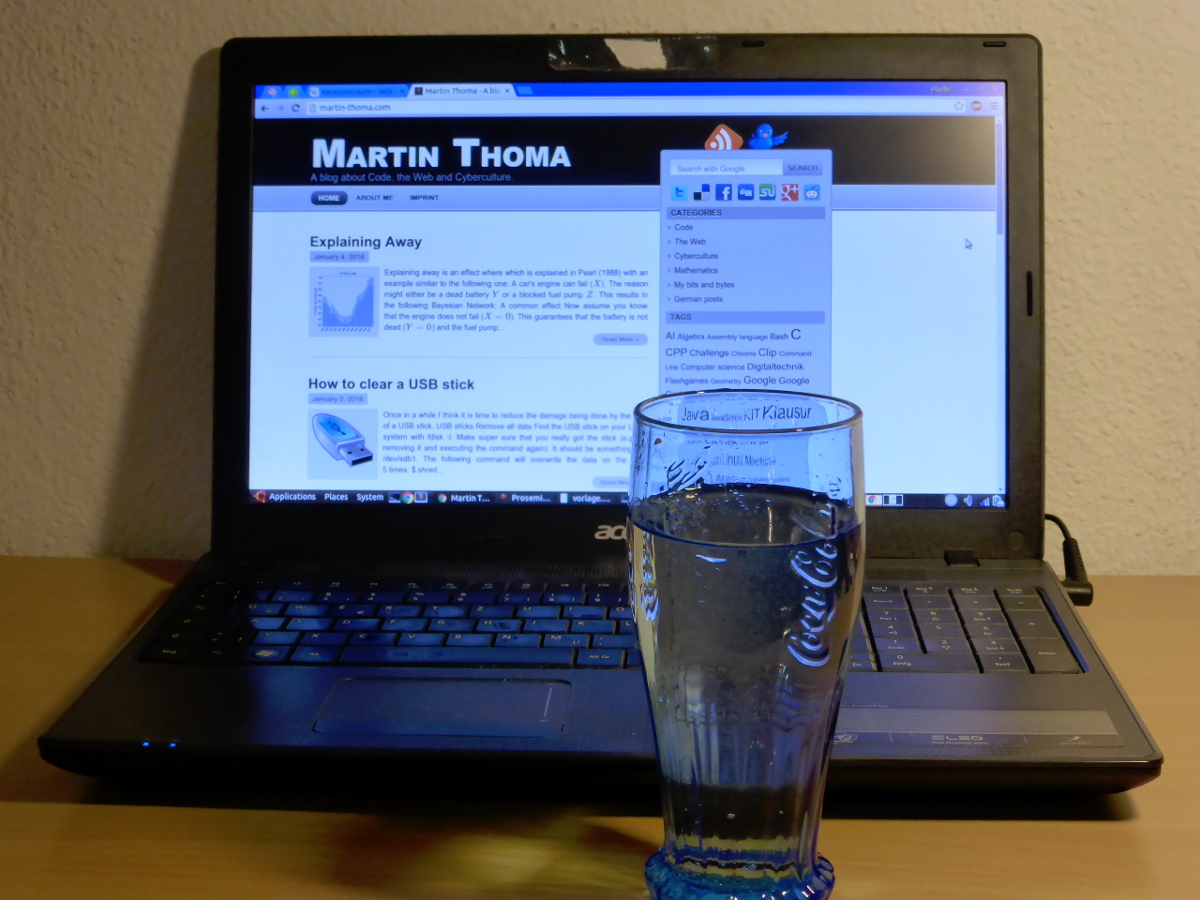
\includegraphics[width=0.45\linewidth, keepaspectratio]{figures/image-segmentation-example.jpg}
}%
\subfigure[Visualization of a found segmentation]{
  \label{fig:segmentation-example-seg}
  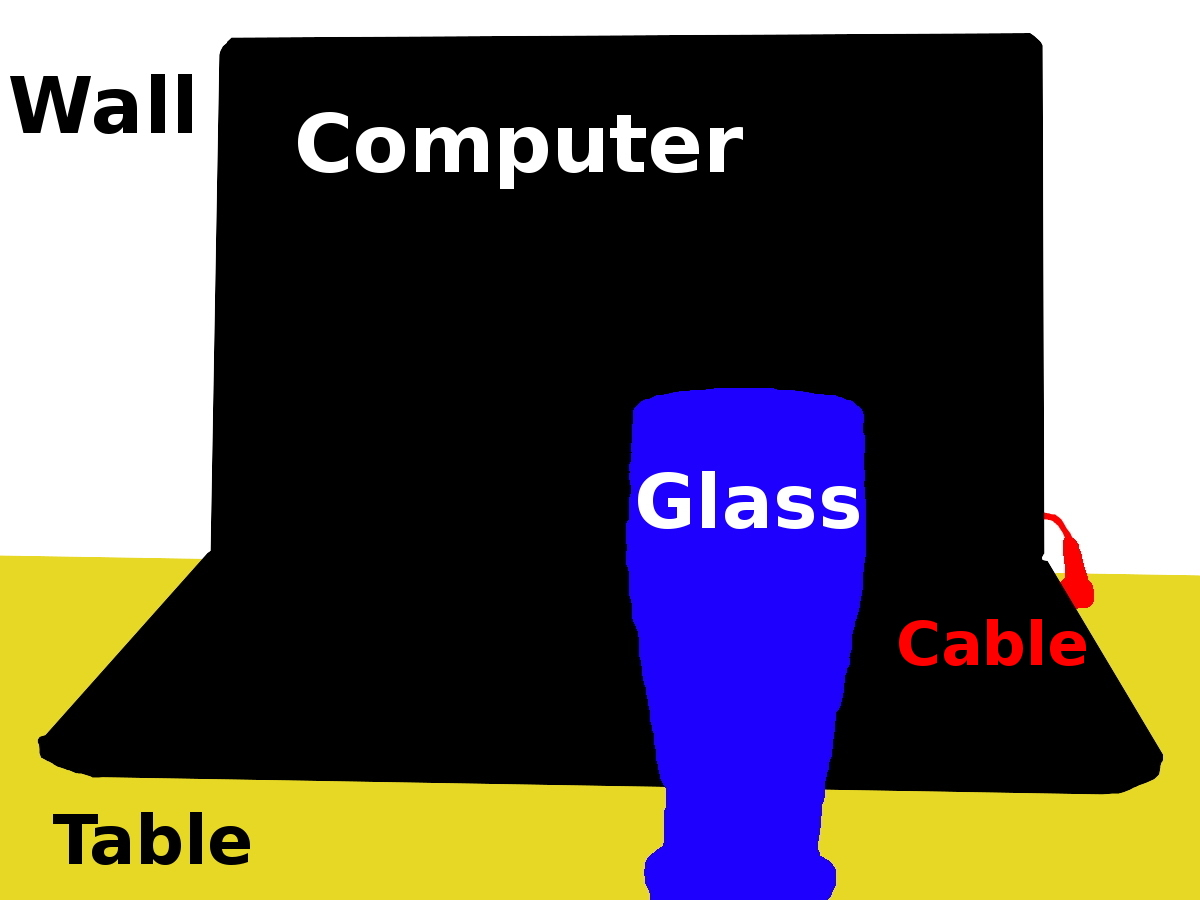
\includegraphics[width=0.45\linewidth, keepaspectratio]{figures/image-segmentation-example-segmented.jpg}
}
\caption{An example of a scene and a possible visualization of a found segmentation.}
\label{fig:segmentation-example}
\end{figure}

However, this can only support the explanation of particular problems or
showcase special situation. For meaningful information about the overall
accuracy, there are a couple of metrics.

For this section, let $k \in \mathbb{N}$ be the number of classes, $n_{ij} \in
\mathbb{N}_0$ with $i,j \in 1, \dots, k$ be the number of pixels which belong to
class~$i$ and were labeled as class~$j$. Let $t_i = \sum_{j=1}^k n_{ij}$ be the
total number of pixels of class~$i$.

One way to compare segmentation algorithms is by the pixel-wise accuracy of the
predicted segmentation as done in many publications
\cite{shotton2006textonboost,csurka2008simple,long2014fully}. This is also
called per-pixel rate and defined as $\frac{\sum_{i=1}^k n_{ii}}{\sum_{i=1}^k
t_i}$. Taking the pixel-wise classification accuracy has two major drawbacks:

\begin{problemnr}
    \item \label{item:problem-large-regions} Tasks like segmenting images for self-driving cars have large regions
          which have one class. This makes achieving classification accuracies
          of more than \SI{30}{\percent} with a priori knowledge only possible.
    \item \label{item:problem-labeling-granularity} The manually labeled images
          could have a more coarse labeling. For example, a human classifier
          could have labeled a region as
          \enquote{car} and the algorithm could have split that region into
          the general \enquote{car} and the more specific \enquote{wheel of a
          car}
\end{problemnr}
\goodbreak
Three accuracy metrics which do not suffer from
\cref{item:problem-large-regions} are used in~\cite{long2014fully}:\nobreak%
\begin{itemize}
    \item \textit{mean accuracy}: $\frac{1}{k} \cdot \sum_{i=1}^n \frac{n_{ii}}{t_i}$
    \item \textit{mean intersection over union}: \hfill\\$\frac{1}{k} \cdot \sum_{i=1}^k \frac{n_{ii}}{t_i + \sum_{j=1}^k n_{ji}-n_{ii}}$
    \item \textit{frequency weighted intersection over union}:
          ${({\sum_{p=1}^k t_p})}^{-1} \sum_i \frac{t_i n_{ii}}{t_i + \sum_{j=1}^k n_{ji} - n_{ii}}$
\end{itemize}

Another problem might be pixels which cannot be assigned one of the known
classes. For this reason, \cite{shotton2006textonboost} makes use of a void
class. This class gets completely ignored for all quality measures. Hence the
total number of pixels is assumed to be $\text{width} \cdot \text{height} - \text{number of void pixels}$.

One way to deal with \cref{item:problem-large-regions} and
\cref{item:problem-labeling-granularity} is giving a confusion matrix as
done in \cite{shotton2006textonboost}. However, this approach is not feasible
if many classes are given.


A lot of other measures for the accuracy of segmentations were proposed for
non-semantic segmentation. One of those accuracy measures is \textit{Normalized
Probabilistic Rand} (NPR) index which was introduced in
\cite{unnikrishnan2005measure} and evaluated in~\cite{celebi2009improved}
on dermoscopy images. Other non-semantic segmentation measures were introduced
in~\cite{martin2001database}, but the reason for creating them seems
to be to deal with the under-defined task description of non-semantic
segmentation. These accuracy measures try to deal with different levels of
coarsity of the segmentation. This is much less of a problem in semantic
segmentation and thus those measures are not explained here.

The $F$-measure is useful for binary classification task such as the KITTI road
segmentation benchmark~\cite{Fritsch2013ITSC} or crypt segmentation as done
by~\cite{cohen2015memory}. It is calculated as \enquote{the harmonic mean of
the precision and recall}~\cite{pantofaru2005comparison}:
\[F_\beta = (1+\beta)^2 \frac{\text{tp}}{(1+\beta^2)\cdot \text{tp}+ \beta^2 \cdot \text{fn} + \text{fp}}\]
where $\beta=1$ is chosen in most cases and \texttt{tp} means \textit{true
positive}, \texttt{fn} means \textit{false negative} and  \texttt{fp} means
\textit{false positive}.


\subsubsection{Speed}%
\label{subsubsec:speed-quality-measure}%
A maximum upper bound on the execution time for the inference on a single image
is a hard requirement for some applications. For example, in the case of
self-driving cars an algorithm which classifies pixel as street or no-street
and thus makes a semantic segmentation, every image needs to be processed
within \SI{20}{\milli\second}~\cite{bittel2015pixel}.

Most papers do not give exact values for the time their application needs. One
reason might be that this is very hardware, implementation and in some cases
even data specific. For example, \cite{hoover1996experimental} notes that their
algorithm needs \SI{10}{\second} on a Sun SparcStation~20. The fastest CPU ever
produced for this system had~\SI{200}{\mega\hertz}. Comparing this directly
with results which were obtained using an Intel~i7-4820K with
\SI{3.9}{\giga\hertz} would not be meaningful.

However, it does still make sense to mention the execution time as well as the
hardware in individual papers. This gives the interested reader the possibility
to estimate how difficult it might be to adjust the algorithm to work in the
required time-constraints. Also, it should be noted if the algorithm can be
executed in parallel as standard \glspl{GPU} on the consumer market can execute
up to 256~kernels in parallel.


\subsubsection{Stability}%
\label{subsubsec:stability-quality-measure}%
The stability of segmentation is a desirable quality measure. One the one hand,
there are some variants of images like slight blurring, Gaussian noise and
similar which should not change the segmentation at all. Also, two images which
show a slight change in perspective should also only result in slight changes
in the segmentation~\cite{pantofaru2005comparison}.

Another desirable stability criterion is parameter choice. If the
segmentation algorithm has hyperparameters, then slightly changing those should
also only result in minor differences of the resulting
segmentations~\cite{pantofaru2005comparison}.


\subsubsection{Memory usage}
Peak memory usage matters when segmentation algorithms get used in devices like
smartphones or cameras, or when the algorithms have to finish in a given time
frame, run on the \gls{GPU} and consume so much memory for single image
segmentation that only the latest graphic cards can be used. However, no
publication we found mentioned the peak memory usage.

%!TEX root = vorlage.tex

\subsection{Datasets}

The computer vision community produced a couple of different datasets which are
publicly available. In the following, only the most widely used ones are
described. An overview over the quantity and the kind of data is given by
\cref{table:segmentation-databases}.


\subsubsection{PASCAL VOC}

The PASCAL\footnote{\textbf{p}attern \textbf{a}nalysis, \textbf{s}tatistical
modelling and \textbf{c}omput\textbf{a}tional \textbf{l}earning, an EU network
of excellence} VOC\footnote{\textbf{V}isual \textbf{O}bject \textbf{C}lasses}
challenge was organized eight times with different datasets: Once every year
from 2005 to 2012~\cite{pascal-voc-2012}. Beginning with~2007, a segmentation
challenge was added~\cite{pascal-voc-2007}.

The dataset consists of annotated photographs from www.flicker.com, a photo
sharing website. There are multiple challenges for PASCAL VOC. The 2012
competition had 5~challenges of which one is a segmentation challenge where
a single class label was given for each pixel.

Although no new competitions will be held, new algorithms can be evaluated on
the 2010, 2011 and 2012 data via
\href{http://host.robots.ox.ac.uk:8080/}{http://host.robots.ox.ac.uk:8080/}

The PASCAL VOC segmentation challenges use the \textit{segmentation over union}
criterion (see \cref{subsec:quality-measures}).


\subsubsection{MSRCv2}

Microsoft Research has published a database of 591 photographs with pixel-wise
annotation of 21~classes: aeroplane, bike, bird, boat, body,
book, building, car, cat, chair, cow, dog, face, flower, grass, road, sheep,
sign, sky, tree, water. Additionally, there is a \texttt{void} label for pixels
which do not belong to any of the 21~classes or which are close to the
segmentation boundary. This allows a \enquote{rough and quick hand-segmentation
which does not align exactly with the object boundaries}~\cite{shotton2006textonboost}.

The dataset is described in~\cite{shotton2006textonboost}.

\subsubsection{Medical Databases}

The Warwick-QU Dataset consists of 165~images with pixel-wise annotation of
5~classes: \enquote{healthy, adenomatous, moderately differentiated,
moderately-to-poorly differentiated, and poorly
differentiated}~\cite{coelho2009nuclear}. This dataset is part of the
Gland Segmentation (GlaS) challenge.

The DIARETDB1~\cite{kalesnykiene2014diaretdb1} is a dataset of 89~images fundus
images. Those images show the interior surface of the eye. Fundus images can
be used to detect diabetic retinopathy. The images have four classes of coarse
annotations: hard and soft exudates, hemorrhages and red small dots.

20~test and additionally 20~training retinal fundus images are available
through the DRIVE data set~\cite{staal2004ridge}. The vessels were annotated.
Additionally, \cite{azzopardi2011detection} added vascular features.


%!TEX root = vorlage.tex

\section{Traditional Approaches}\label{sec:traditional-approaches}%
Image segmentation algorithms which use traditional approaches, hence don't
apply neural networks and make heavy use of domain knowledge, are wide-spread
in the computer vision community. Features which can be used for segmentation
are described in \cref{subsec:features}, a very brief overview of unsupervised,
non-semantic segmentation is given in
\cref{subsec:unsupervised-traditional-segmentation}, Random Decision
Forests are described in \cref{subsec:random-forests}
%, Markov Random Fields in \cref{subsec:markov-random-fields}
 and \glspl{SVM} in
\cref{subsec:trad-SVM}.
Postprocessing is covered in \cref{subsec:post-processing-methods}.

It should be noted that algorithms can use combination of methods. For example,
\cite{tighe2014scene} makes use of a combination of a \gls{SVM} and a
\gls{MRF}.

% TODO: The respective advantages of the classifiers are discussed in
% \cref{subsec:traditional-approaches-discussion}.

%!TEX root = vorlage.tex

\subsection{Features and Preprocessing methods}\label{subsec:features}%
The choice of features is very important in traditional approaches.
The most commonly used features are explained in the following.

\subsubsection{Pixel Color}
Pixel color in different image spaces (e.g. 3~features for RGB, 3~features for
HSV, 1~feature for the gray-value). A typical image is in the RGB color space,
but depending on the classifier and the problem another color space might
result in better segmentations. RGB, YcBcr, HSL, Lab and YIQ are some examples
used by \cite{cohen2015memory}. No single color space has been proven to be
superior to all others in all contexts~\cite{cheng2001color}. However, the most
common choices seem to be RGB and HSI. Reasons for choosing RGB is simplicity
and the support by programming languages, whereas the choice of the HSI color
space might make it simpler for the classifier to get invariant to
illumination. One reason for choosing CIE-L*a*b* color space is that it
approximates human perception of brightness~\cite{kasson1992analysis}. It
follows that choosing the L*a*b color space helps algorithms to detect
structures which are seen by humans. Another way of improving the structure
within an image is histogram equalization, which can be applied to improve
contrast~\cite{pizer1987adaptive,4228537}.

\subsubsection{Histogram of oriented Gradients}
\Gls{HOG} features interpret the image as a discrete function
$I: \mathbb{N}^2 \rightarrow \Set{0, \dots, 255}$ which maps the position $(x,
y)$ to a color. For each pixel, there are two gradients: The partial derivative
of $x$ and $y$. Now the original image got transformed to two feature maps of
equal size which represents the gradient. These feature maps are splitted into
patches and a histogram of the directions is calculated for each patch.
\gls{HOG} features were proposed in~\cite{1467360} and are used
in~\cite{bourdev2010detecting,felzenszwalb2010object}.


\subsubsection{SIFT}
\Gls{SIFT} feature descriptors find keypoints in an image. The image patch of
the size $16 \times 16$ around the keypoint is taken. This patch is divided in
$16$ distinct parts of the size $4 \times 4$. For each of those parts a
histogram of 8~orientations is calculated similar as for \gls{HOG} features.
This results in a 128-dimensional feature vector for each keypoint.

\Gls{SIFT} is described in detail in~\cite{raey}.


\subsubsection{BOV}
\Gls{BOV}, also called \textit{bag of keypoints}, is based on vector
quantization. Similar to \gls{HOG} features, \gls{BOV} features are histograms
which count the number of occurrences of certain patterns within a patch of the
image. \Gls{BOV} are described in~\cite{csurka2004visual} and used in
combination with \gls{SIFT} feature descriptors in~\cite{csurka2008simple}.


\subsubsection{Poselets}
\textit{Poselets} were used successfully
in~\cite{bourdev2010detecting,brox2011object}. Those features rely on manually
added extra keypoints such as \enquote{right shoulder}, \enquote{left
shoulder}, \enquote{right knee} and \enquote{left knee}. They were originally
used for human pose estimation. Finding those extra keypoints is easily
possible for well-known image classes like humans. However, it is difficult for
classes like airplanes, ships, organs or cells where the human annotators do
not know the keypoints. Additionally, the keypoints have to be chosen for every
single class. There are strategies to deal with those problems like
viewpoint-dependent keypoints.


\subsubsection{Textons}\label{subsubsec:textons}
A \textit{texton} is the minimal building block of vision. The computer vision
literature does not give a strict definition for textons, but edge detectors
could be one example. One might argue that deep learning techniques with
\glspl{CNN} learn textons in the first filters.

An excellent explanation of textons can be found in~\cite{zhu2005textons}.


\subsubsection{Dimensionality Reduction}
High-resolution images have a lot of pixels. Having one or more feature per
pixel results in many features. This makes training difficult while the higher
resolution might not contain much more information. A simple approach to deal
with this is downsampling the high-resolution image to a low-resolution
variant. Another way of doing dimensionality reduction is \gls{PCA}, which is
applied by~\cite{chen2011pixel}. The idea behind \gls{PCA} is to find a
hyperplane on which all feature vectors can be projected with a minimal loss of
information. A detailed description of \gls{PCA} is given
by~\cite{smith2002tutorial}.

One problem of \gls{PCA} is the fact that it does not distinguish different
classes. This means it can happen that a perfectly linearly separable set of
feature vectors gets not separable at all after applying \gls{PCA}.

There are many other techniques for dimensionality reduction. An overview and
a comparison over some of them is given by~\cite{van2009dimensionality}.

%!TEX root = vorlage.tex

\subsection{Unsupervised Segmentation}%
\label{subsec:unsupervised-traditional-segmentation}%

Unsupervised segmentation algorithms can be used in supervised segmentation as
another source of information or to refine a segmentation. While unsupervised
segmentation algorithms can never be semantic, they are well-studied and
deserve at least a very brief overview.

Semantic segmentation algorithms store information about the classes they were
trained to segment while non-semantic segmentation algorithms try to detect
consistent regions and region boundaries.

\subsubsection{Clustering Algorithms}
The $k$-means algorithm is a general-purpose clustering algorithm which
requires the number of clusters to be given beforehand. Initially, it places
the $k$ centroids randomly in the feature space. Then it assigns each
data point to the nearest centroid, moves the centroid to the center of the
cluster and continues the process until a stopping criterion is reached. A
faster variant is described in \cite{hartigan1975clustering}.

$k$-means was applied by~\cite{chen1998image} for medical image segmentation.

Another clustering algorithm is the mean-shift algorithm which was introduced
by~\cite{comaniciu2002mean} for segmentation tasks. The algorithm finds the
cluster centers by initializing centroids at random seed points and iteratively
shifting them to the mean coordinate within a certain range. Instead of taking
a hard range constraint, the mean can also be calculated by using any kernel.
This effectively applies a weight to the coordinates of the points. The mean
shift algorithm will give cluster centers at positions with a highest local
density of points.


\subsubsection{Graph Based Image Segmentation}%
\label{subsec:graph-based-image-segmentation}%
Graph-based image segmentation algorithms typically interpret pixels as
vertices and an edge weight is a measure of dissimilarity such as the
difference in color~\cite{felzenszwalb2004efficient,FelzenszwalbGraphCode}.
There are several different candidates for edges. The 4-neighborhood (north,
east, south west) or an 8-neighborhood (north, north-east, east, south-east,
south, south-west, west, north-west) are plausible choices.
One way to do the cuts is by building a minimum spanning tree and removing
edges above a threshold. This threshold can either be constant, adapted to the
graph or adjusted by the user. After the edge-cutting step, the connected
components are the segments.

A graph-based method which got the \nth{2} rank in the Pascal VOC 2010
challenge~\cite{everingham2010pascal} is described
in~\cite{carreira2010constrained}. The system makes heavy use of the multi-cue
contour detector globalPb~\cite{4587420} and needs about \SI{10}{\giga\byte}
of main memory~\cite{Carreira2011}.


\subsubsection{Random Walks}

Random walks belong to the graph-based image segmentation algorithms. Random
walk image segmentation usually works as follows: Some seed points are placed
on the image for the different objects in the image. From every single pixel,
the probability to reach the different seed points by a random walk is
calculated. This is done by taking image gradients as described in
\cref{subsec:features} for \gls{HOG} features. The class of the pixel is the
class of which a seed point will be reached with highest probability. At first,
this is an interactive segmentation method, but it can be extended to be
non-interactive by using another segmentation methods output as seed points.

It was shown in~\cite{meilpa2001learning} that normalized cuts
(NCuts)~\cite{shi2000normalized} can be expressed with random walks.


\subsubsection{Active Contour Models}

\Glspl{ACM} are algorithms which segment images roughly along edges, but try
also try to find a border which is smooth. This is done by defining a so called
\textit{energy function} which will get minimized. They were initially
described in~\cite{kass1988snakes}. \Glspl{ACM} can be used to segment an image
or to refine segmentation as it was done in~\cite{atkins1998fully} for brain
\gls{MR} images.


\subsubsection{Watershed Segmentation}\label{subsec:watershed}
The watershed algorithm takes a grayscale image and interprets it as a height
map. Low values are catchment basins and the higher values between two
neighboring catchment basins is the watershed. The catchment basins should
contain what the developer wants to capture. This implies that those areas
must be dark on grayscale images. The algorithm starts to fill the basins from
the lowest point. When two basins get connected, a watershed is found. The
algorithm stops when the highest point is reached.

A detailed description of the watershed segmentation algorithm is given
in~\cite{roerdink2000watershed}.

The watershed segmentation was used in~\cite{1260033} to segment white blood
cells. As the authors describe, the segmentation by watershed transform has
two flaws: Over-segmentation due to local minima and thick watersheds due to
plateaus.

%!TEX root = vorlage.tex

\subsection{Random Decision Forests}\label{subsec:random-forests}

Random Decision Forests were first proposed in~\cite{ho1995random}. This type
of classifier applies techniques called \textit{ensemble learning}, where
multiple classifiers get trained and a combination of their hypotheses is
used. One ensemble learning technique is the \textit{random subspaces} method
where each classifier gets trained on a random subspace of the feature~space.
Another ensemble learning technique is \textit{bagging}, which is training the
trees on random subsets of the training~set. In the case of Random Decision
Forests, the classifiers are decision trees. A decision tree is a tree where
each inner node uses one or more features to decide in which branch to descend.
Each leaf is a class.

A strength of Random Decision Forests compared to many other classifiers like
\glspl{SVM} and neural networks is that the scale of measure of the features
(nominal, ordinal, interval, ratio) can be arbitrary.

Random decision trees were extensively studied in the past 20~years and a
multitude of training algorithms has been proposed (e.g. ID3
in~\cite{quinlan1986induction}, C4.5 in~\cite{quinlan2014c4}). Possible
training hyperparameters are the measure to evaluate the \enquote{goodness of
split}~\cite{raey89empirical}, the number of decision trees being used, and if
the depth of the trees is restricted. Typically in the context of
classification, random decision trees are trained by adding new nodes until
each leaf contains only nodes of a single class or until it is not possible to
split further. This is called a \textit{stopping criterion}.

There are two typical training modes: \textit{Central axis projection} and
\textit{perceptron training}. In training, for each node a hyperplane is
searched which is optimal according to an error function.

Random Decision Forests with texton features (see \cref{subsubsec:textons}) are
applied in~\cite{shotton2008semantic} for segmentation. In the~\cite{MSCR-db}
dataset, they report a per-pixel accuracy rate of \SI{66.9}{\percent} for their
best system. This system needs \SI{415}{\milli\second} for the segmentation of
$\SI{320}{\pixel} \times \SI{213}{\pixel}$ images on a single
\SI{2.7}{\giga\hertz} core. On the Pascal VOC~2007 dataset, they report an
average per-pixel accuracy for their best segmentation system
of~\SI{42}{\percent}.

% %!TEX root = vorlage.tex

\subsection{Markov Random Fields}\label{subsec:markov-random-fields}
\Glspl{MRF} are undirected probabilistic graphical models. In the associated
graph $G=(\mathcal{V}, \mathcal{E})$, nodes represent random variables and
edges represent conditional dependencies. Inference is done with the \gls{MAP}
estimation and training with a maximum likelihood approach (with gradient
ascent, see L-BFGS~\cite{liu1989limited}) or \gls{ICM}~\cite{10.2307/2345426}.
\Gls{MAP} is a substitute for \gls{MLE}.

Typically, random variables $\mathbf{y}$ represent the class of a single pixel,
random variables $\mathbf{x}$ represent a pixel values
and edges represent pixel neighborhood in computer vision problems segmentation problems
where \glspl{MRF} are used. The pixel neighborhood might either be a
4-neighborhood (north, east, south west) or an 8-neighborhood (north,
north-east, east, south-east, south, south-west, west, north-west).

For example, say $\mathbf{x}$ is the feature vector from an image, $\mathbf{y}$
is the vector of random variables. Then the conditional probability of $\mathbf{y}$
given $\mathbf{x}$ can be expressed as
\[P(\mathbf{y}|\mathbf{x}) = \frac{1}{Z(\mathbf{x})} \exp(-E(\mathbf{y};\mathbf{x}))\]
where $Z(\mathbf{x}) = \sum_{\mathbf{y}} \exp(-E(\mathbf{y};\mathbf{x}))$ is
a normalization term called the \textit{partition function}.

Typically, the energy function $E$ is of the structure

\[E(\mathbf{y}, \mathbf{x}) = \sum_{i \in \mathcal{V}} \psi_i^U (y_i; \mathbf{x}) + \sum_{ij \in \mathcal{E}} \psi_{ij}^P(y_i, y_j, \mathbf{x}) + \sum_{c \in \mathcal{C}} \psi_c^H(\mathbf{y}_c; \mathbf{x})\]

where $\psi_i^U$ represents unary terms, $\psi_{ij}^P$ represents pairwise
terms and $\psi_c^H$ represents higher-order terms. $\mathcal{C}$ is the set
of all cliques in $G$.


\Glspl{MRF} are a very wide-spread model in computer vision. Excellent
introductions to \glspl{MRF} are given by
\cite{blake2011markov,murphy2012machine}.


% Where / how it was used.
Grid-like / pairwise \gls{MRF} is used in~\cite{rother2004grabcut}.

Other \glspl{MRF}: \cite{zhang2001segmentation} and \cite{moser2012markov}.

\cite{shotton2006textonboost} uses a 4-connected grid.

\Gls{PGM} have some problems:

\begin{itemize}
    \item Exact inference, that means computing \(P_\Phi(X=x)\), given a
          \Gls{PGM} $P_\Phi$ and a variable \(X\) as well as a value \(x \in Val(X)\),
          is NP-hard.
    \item Approximate inference is NP-Hard
\end{itemize}

% Characterizations of MRF:
% Label space: binary vs multi-label; homogeneous vs heterogeneous
% Order: unary vs pairwise vs higher-order
% Structure: chain vs tree vs grid vs general graph; neighborhood size
% Potentials: submodular, convex, compressible



% Markov Random Fields (A Rough Guide)
% http://www.mee.tcd.ie/~sigmedia/pmwiki/uploads/Main.Tutorials/mrf_tutorial.pdf

% Markov Random Fields and Stochastic Image Models
% http://cis-linux1.temple.edu/~latecki/Courses/RobotFall08/Papers/MRFBauman.pdf

% Markov Random Fields
% http://signal.ee.psu.edu/mrf.pdf

% Markov Random Fields for Computer Vision (Part 1)
% http://users.cecs.anu.edu.au/~sgould/papers/part1-MLSS-2011.pdf  --- very nice!


% Markov Random Fields and Stochastic Image Models
% https://engineering.purdue.edu/~bouman/publications/tutorials/mrf_tutorial/view.pdf


% Markov Random Fields in Image Segmentation
% http://web.inf.u-szeged.hu/~ssip/2011/PDF/ssip2011_Kato.pdf

% Book about markov random fields in computer vision:
% https://mitpress.mit.edu/sites/default/files/titles/content/9780262015776_sch_0001.pdf


\Glspl{CRF} and Boltzmann Machines are a variations of Markov random fields.

% Markov Random Field Image Models and Their Applications to Computer Vision
% http://www.mathunion.org/ICM/ICM1986.2/Main/icm1986.2.1496.1517.ocr.pdf
%
% Segmentation of brain MR images through a hidden Markov random field model
% and the expectation-maximization algorithm \cite{zhang2001segmentation}

% In short: specify locally and model globally.

% define only local properties. allows by transitivity to get a model
% for global properties.


% \begin{itemize}
%     \item What is your set of random models? (e.g. Ising model: one for each pixel)
%           \begin{itemize}
%               \item Irving-Model: \cite{boykov2000interactive}
%               \item Potts-Model: \cite{boykov2001fast}
%           \end{itemize}
% \end{itemize}

% On those, define an undirected hypergraph $G(V, E)$. $V$ are pixels, $E$ is
% typically defined by neighboring pixels.

% good:

% \begin{itemize}
%     \item Convenient modeling:Just write down energy function (in some cases)
%           do define entire model
%     \item fast inference (only 1 or 2 variants)
%     \item sometimes good performance
% \end{itemize}

% bad:

% \begin{itemize}
%     \item learning is difficult
% \end{itemize}


% From \cite{yang2012layered}:

% > In contrast, semantic segmentation models have largely been built on top of
% Markov Random Field (MRF) models which enforce smoothness across pixel labels

% \begin{itemize}
%     \item A. Torralba, K. Murphy, and W. Freeman, “Contextual Models for
%           Object Detection Using Boosted Random Fields,” Proc. Advances in
%           Neural Information Processing Systems, 2004.
%     \item S. Kumar and M. Hebert, “A Hierarchical Field Framework for
%           Unified Context-Based Classification,” Proc. 10th IEEE Int’l Conf.
%           Computer Vision, vol. 2, 2005.
%     \item Z. Tu, “Auto-Context and Its Application to High-Level Vision
%           Tasks,” Proc. IEEE Conf. Computer Vision and Pattern Recognition,
%           2008.
% \end{itemize}


\subsection{Conditional Random Fields}\label{subsec:conditional-random-fields}

\Glspl{CRF} are \glspl{MRF} where all clique potentials are conditioned on
input features~\cite{murphy2012machine}. This means, instead of learning the
distribution $P(\mathbf{Y}, \mathbf{X})$, the task is reformulated to learn the
distribution $P(\mathbf{Y}| \mathbf{X})$. One consequence of this reformulation
is that \glspl{CRF} need much less parameters as the distribution of $X$ does
not have to be estimated. Another advantage of \glspl{CRF} compared to
\glspl{MRF} is that no distribution assumption about $X$ has to be made.

Formally, a \gls{CRF} is a set of factors

\[\Phi = \Set{\phi_1(\mathbf{D}_1), \dots, \phi_k(\mathbf{D}_k)}\]

together with a normalization function called \textit{partition function} $Z_\Phi$:
\[Z_\Phi(\mathbf{X}) = \sum_{\mathbf{Y}} \tilde{P_\Phi} (\mathbf{X}, \mathbf{Y})\]

which results in the joint probability distribution

\[P_{\Phi}(\mathbf{Y} | \mathbf{X}) = \frac{1}{Z_\Phi(\mathbf{X})} \prod_{i=1}^k \phi_i(\mathbf{D}_i)\]


\Glspl{CRF} are used in \cite{multiscale04,shotton2006textonboost}.

\Glspl{CRF} as described in~\cite{associative09} have reached top performance
in PASCAL VOC 2010~\cite{VOC2010Results}.

% An Introduction to Conditional Random Fields
% http://homepages.inf.ed.ac.uk/csutton/publications/crftutv2.pdf

A method similar to \glspl{CRF} was proposed in~\cite{gonfaus2010harmony}.
The system of Gonfaus~et.al. ranked~\nth{1} by mean accuracy in the segmentation
task of the PASCAL VOC 2010 challenge~\cite{everingham2010pascal}.
 TODO
%!TEX root = vorlage.tex

\subsection{SVMs}\label{subsec:trad-SVM}%

\Glspl{SVM} are well-studied binary classifiers which can be described by four
central ideas. For those ideas, the training data is represented as
$(\mathbf{x}_i, y_i)$ where $\mathbf{x}_i$ is the feature vector and $y_i \in
\Set{-1, 1}$ the binary label for training example $i \in \Set{1, \dots, m}$.


\begin{enumerate}
    \item If data is linearly separable, it can be separated by a hyperplane.
          There is one hyperplane which maximizes the distance to the
          datapoints. This hyperplane should be taken:\\
          \begin{equation*}
          \begin{aligned}
              \minimize_{\mathbf{w}, b}\,&\frac{1}{2} \|\mathbf{w}\|^2\\
              \text{s.t. }& \forall_{i=1}^m y_i \cdot \underbrace{(\langle \mathbf{w}, \mathbf{x}_i\rangle + b)}_{\mathclap{\sgn \text{ applied to this gives the classification}}} \geq 1
          \end{aligned}
          \end{equation*}
    \item Even if the underlying process which generates the features for the
          two classes is linearly separable, noise can make the data not
          separable. The introduction of \textit{slack variables} to relax the
          requirement of linear separability solves this problem. The trade-off
          between accepting some errors and a more complex model is weighted by
          a parameter $C \in \mathbb{R}_0^+$. The bigger $C$, the more errors
          are accepted. The new optimization problem is:
          \begin{equation*}
          \begin{aligned}
              \minimize_{\mathbf{w}}\,&\frac{1}{2} \|\mathbf{w}\|^2 + C \cdot \sum_{i=1}^m \xi_i\\
              \text{s.t. }& \forall_{i=1}^m y_i \cdot (\langle \mathbf{w}, \mathbf{x}_i\rangle + b) \geq 1 - \xi_i
          \end{aligned}
          \end{equation*}
    \item The primal problem is to find the normal vector $\mathbf{w}$ and the
          bias $b$. The dual problem is to express $\mathbf{w}$ as a linear
          combination of the training data $\mathbf{x}_i$:
          \[\mathbf{w} = \sum_{i=1}^m \alpha_i y_i \mathbf{x}_i\]
          where $y_i \in \Set{-1, 1}$ represents the class of the training
          example and $\alpha_i$ are Lagrange multipliers. The usage of
          Lagrange multipliers is explained with some examples
          in~\cite{smithlagrange}. The usage of the Lagrange multipliers
          $\alpha_i$ changes the optimization problem depend on the
          $\alpha_i$ which are weights for the feature vectors. It turns
          out that most $\alpha_i$ will be zero. The non-zero weighted vectors
          are called \textit{support vectors}.

          The optimization problem is now, according to~\cite{burges1998tutorial}:
          \begin{equation*}
          \begin{aligned}
              \maximize_{\mathbf{w}}\,& \sum_{i=1}^m \alpha_i - \frac{1}{2} \sum_{i=1}^m \sum_{j=1}^m \alpha_i \alpha_j y_i y_j \langle \mathbf{x}_i, \mathbf{x}_j \rangle\\
              \text{s.t. } & \forall_{i=1}^m 0 \leq \alpha_i \leq C\\
              \text{s.t. } & \sum_{i=1}^m \alpha_i y_i = 0
          \end{aligned}
          \end{equation*}
    \item Not every dataset is linearly separable. This problem is approached
          by transforming the feature vectors $\mathbf{x}$ with a non-linear
          mapping $\Phi$ into a higher dimensional (probably
          $\infty$-dimensional) space. As the feature vectors $\mathbf{x}$
          are only used within scalar product
          $\langle \mathbf{x}_i, \mathbf{x}_j \rangle$, it is not necessary to
          do the transformation. It is enough to do the calculation
          \[K(\mathbf{x}_i, \mathbf{x}_j) = \langle \mathbf{x}_i, \mathbf{x}_j \rangle\]

          This function $K$ is called a \textit{kernel}. The idea of never
          explicitly transforming the vectors $\mathbf{x}_i$ to the higher
          dimensional space is called the \textit{kernel trick}. Common kernels
          include the polynomial kernel
          \[K_P(\mathbf{x}_i, \mathbf{x}_j) = (\langle \mathbf{x}_i, \mathbf{x}_j \rangle + r)^p\]
          of degree $p$ and coefficient $r$, the Gaussian \gls{RBF} kernel
          \[K_{\text{Gauss}}(\mathbf{x}_i, \mathbf{x}_j) = e^{\frac{-\gamma\|\mathbf{x}_i - \mathbf{x}_j\|^2}{2 \sigma^2}}\]
          and the sigmoid kernel
          \[K_{\text{tanh}}(\mathbf{x}_i, \mathbf{x}_j) = \tanh(\gamma \langle \mathbf{x}_i, \mathbf{x}_j \rangle - r)\]
          where the parameter $\gamma$ determines how much influence single
          training examples have.
\end{enumerate}

The described \glspl{SVM} can only distinguish between two classes. Common
strategies to expand those binary classifiers to multi-class classification is
the \textit{one-vs-all} and the \textit{one-vs-one} strategy. In the one-vs-all
strategy $n$ classifiers have to be trained which can distinguish one of the $n$
classes against all other classes. In the one-vs-one strategy $\frac{n^2 - n}{2}$
classifiers are trained; one classifier for each pair of classes.

A detailed description of \glspl{SVM} can be found in~\cite{burges1998tutorial}.

\Glspl{SVM} are used by \cite{yang2012layered} on the 2009 and 2010 PASCAL
segmentation challenge~\cite{everingham2010pascal}. They did not hand their
classifier in to the challenge itself, but calculated an average rank~of~7
among the different categories.

\cite{felzenszwalb2010object} also used an \gls{SVM} based method with \gls{HOG}
features and achieved the \nth{7}~rank in the 2010 PASCAL segmentation
challenge by mean accuracy. It needs about \SI{2}{\second} on a
\SI{2.8}{\giga\hertz} 8-core Intel processor.

%!TEX root = vorlage.tex

\subsection{Post-processing methods}\label{subsec:post-processing-methods}%
Post-processing methods are an important part of traditional pixel-level
segmentation approaches. They refine a found segmentation and remove obvious
errors. For example, the morphological operations \textit{opening} and
\textit{closing} can remove noise. The opening operation is a dilation followed
by a erosion. This removes tiny segments. The closing operation is a erosion
followed by a dilation. This removes tiny gaps in otherwise filled regions.
They were used in~\cite{chen1998image} for biomedical image segmentation.

Another way of refinement of the found segmentation is by adjusting the
segmentation to match close edges. This was used in~\cite{brox2011object} with
an ultra-metric contour map~\cite{arbelaez2009contours}.

Active contour models are another example of a post-processing
method~\cite{kass1988snakes}.


% TODO:
% \subsection{Discussion}\label{subsec:traditional-approaches-discussion}%
% According to \cite{pantofaru2005comparison}, the mean shift algorithm produces
% segmentations that correspond well to human perception, but it is sensitive to
% its parameters. Depending on them, different granularities of the segmentation
% can be achieved. \cite{pantofaru2005comparison} draws the conclusion, that
% the segmentations found by the graph based image segmentation approach
% in \cite{felzenszwalb2004efficient} are inferior to the segmentations found
% by the mean shift algorithm described in \cite{comaniciu2002mean}.

%%!TEX root = vorlage.tex
% Marvin Teichmann

%TODO: Type of MLP
\section{Neural Networks for Segmentation}\label{sec:fcn}

After the overwhelming successes of \Glspl{DCNN} in image classification, there as been a lot of effort to apply this models to further computer vision tasks. Early ideas include the use of \Glspl{CNN} based classifiers in combination with traditional classifiers \cite{RNN}. Other authors used the idea descripted in \cref{sec:tasks} to tackle segmentation as pixel-wise classification problem using a sliding-window approach together with a classification network \cite{fast_scanning}, \cite{overfeat}, \cite{bktt} \cite{highly}. These authors profit from the inherent sliding window efficenty of \Glspl{CNN}, descripted in \cref{sec:convnet}. A recent break-trough has been archieved with the novel \gls{FCN} \cite{fcn} architectures. \Gls{FCN} are an architecture specifically designed for Semantic Segmentation. \Gls{FCN} combine the sliding window efficenty with a deconvolution architecture for upsampling and a transfer learning approach. \glspl{FCN} and there deeper successors \cite{CRF1}, \cite{deconv1} \cite{googleSeg} are currently the state-of-the art in several semantic segmentation benchmarks. We will descripe the mechanics behind \glspl{FCN} in detail in \cref{sec:fcn_detail}.


\iffalse

As described in \Cref{sec:tasks} Semantic Segmentation can be views as a spatial version of classification, where a classification model can be transfered into a segmentation model using a sliding window approach. In \glspl{CNN} sliding window can be carried out very efficiently. Most CNN based segmentation approaches are using this insight to build models on the shoulders of AlexNet and its deeper successors. 

\fi

\subsection{Sliding Window efficiency in CNNs} \label{sec:convnet}

Opposed to other classification approaches ConvNets are inherently effecient when applied in sliding window fashion. Their translation invariant structure allows to benifit from computation on overlapping patches on the images. Of high practical relevants is also, that the result itselfe will be a ConvNet, that means any ConvNet $C$ can easily be transformed in a ConvNet $C'$, whose output is equal to applying $C$ in sliding window fashion. This idea can hence be very efficently implemented in any ConvNet framework, without much efford. The only downside is, that $C'$ will have a stride $s$ equal to the product of all strides in $C$.

The reason for the efficienty is, that translation invariant computing is computational traceable. Let $F, G$ function, computing a layer as defined in \cref{sec:cnn_not}. Let $f,g$ kernels corresponding with sizes $k,k'$ and stride $s,s'$, corresponding to $F, G$ respectively. Than $F \circ G$ is obtained by the kernel $f \circ g$, which has kernel size $k + (k-1) s'$ using stride $s \cdot s'$. For networks only consisting of convolution and pooling layers one can therefore simple increase the size of the input layer at evaluation time. The output will be equivalent to apply the original network in sliding-window fashion. Common ConvNet architectures typically have one or more fully-connected layer producing the final classification output. This layers can be replaced by convolutional layers using the trick descripted in \cref{sec:fully_connected}. 

The main downside of this approach is the stride of the overall output stride. The output image of the transformed ConvNet $C'$ will be an low resolution image. The input image will be downsampled by a factor of $s$ corresponding to the product of all strides beeing applied in $C'$. On most network architectures $s$ becomes quite large, e.g. $32$ on VGG16, a network using pooling very cautiously. 

To avoid downsampling while still profiting from the sliding window efficiently of \glspl{CNN} it is possible to use shift-and-stitch. Each layer which is associated with an stride $s$ is feeded with $s^2$ shifted versions of the input. (Each with a different shift in $x$ or $y$ dimension). The output can than be stitched together in order to obtain an image of original resolution. The result is than equivalent in applying sliding-window with stride 1. However the computational advatage of applying strided pooling is lost in the procedure (while the model advantage remains). Fast-scanning \cite{fast_scanning} descripes a trick to efficiently perform this computation.  This idea is used in several publications \cite{overfeat,huval}.


\subsection{FCN} \label{sec:fcn_detail}

The \glspl{FCN} \cite{fcn} Architecture builds up on the ideas presented of \cref{sec:convnet}. Similar to earlier approaches they are using existing classification networks and transform them into segmentation networks using the inherent sliding-window efficientcy of ConvNets. However opposed to earlier approach they are not trying to avoid downsampling as part of the progress, but they are using a trainable upsampling layer to archive high resolution output. Further ingredients of their approach is a skip-architecture to  preserve fine-grained information and a transfer-learning approach making it possible to train a very deep net.


\subsubsection{Deconvolution} Todo: detailed explanation of deconvolution



\subsubsection{Skip-Architecture}



\subsubsection{Transfer Learning} One of the strengthes of the FCN approach is the use of transfer learning. Training is done in two steps. First the classification network is done using weakly annotated data (i.e. classification labels). Afterwards the last layer of the architecture is replaced by a deconvolution layer. Only than the Network is fine-tuned on segmentation data. Usually weakly labeled data is much cheaper to obtain than fully labeled segmentation data making this approach very attractive for a lot of applications.


In the publication several the FCN approach was applied to AlexNet, VGG16 and GoogLeNet. The best results where achieved on VGG16. A possible explanation for this is, that VGG16 uses stride and pooling most cautiously perserving spatial information best.




\subsection{Extensions of FCN}

Several extensions of FCN have been proposed. All of are based on VGG16. The main differentses between the approaches are how the how upsambling is performed. 

Several Authors have combined FCNs with CRFs very succesfully. Zheng et. al \cite{CRF1} and Chen et at. \cite{CRF2} improved the results of Long et. al \cite{fcn} by applying \gls{CRF} on top of the FCN architecture. 

\cite{deconv1} and \cite{segnet} proposed a slightly different approach. The designed a deep decoding network to performe the upsampling. Where each layer of the decoding network corresponds to a pooling layer of the VGG network. The upsampling itselfe is not trained but computed directly using the max pooling indezies. Trained convolution layers are used between the upsampling operations to refine the results. The main downside of this approaches is, that the networks need a large amount of strong labeled data as they are fully trained end-to-end. This problem is relaxed in \cite{decoupled}, by introducing transfer-learning to deep deconvolution networks.






%!TEX root = vorlage.tex

\section{Neural Networks for Semantic Segmentation}\label{sec:nn}

Artificial neural networks are classifiers which are inspired by neurons.
Every single neuron has some inputs which it sums up, applies a so called
\textit{activation function} to it and gives an output. Those neurons can take
either a feature vector as input or the output of other neurons. In this way,
they build up feature hierarchies.

The parameters they learn are the weights. They get learned by gradient
descent. To do so, an error function --- usually cross-entropy or mean squared
error --- is necessary. For the gradient descent algorithm, one sees the
labeled training data as given, the weights as variables and the error function
as a surface in this weight-space. Minimizing the error function in the weight
space adapts the neural network to the problem.

There are lots of ideas around neural networks like regularization, better
optimization algorithms, automatically building up architectures, design
choices for activation functions. I will not go into detail here, but I want to
outline some of the mayor breakthroughs.

\Glspl{CNN} are neural networks which learn image filters. They drastically
reduce the number of parameters which have to be learned while being still
general enough for the problem domain of images. This was shown by Alex
Krizhevsky~et~al. in~\cite{krizhevsky2012imagenet}. One major idea was a clever
regularization called \textit{dropout training}, which set the output of neurons
while training randomly to zero. Another contribution was the usage of an activation
function called \textit{rectified linear unit}:
\[\varphi_{\text{ReLU}}(x) = \max(0, x)\]
Those are much faster to train than the commonly used sigmoid activation functions
\[\varphi_{\text{Sigmoid}}(x) = \frac{1}{e^{-x} + 1}\]
Krizhevsky~et~al. implemented those ideas and ran it participated in the
\gls{ILSVRC}. The best other system, which used SIFT features and Fisher
Vectors, had a performance of about \SI{25.7}{\percent} while the network by
Alex Krizhevsky~et~al. got \SI{17.0}{\percent} error rate on the ILSVRC-2010.
As a preprocessing step, they downsampled all images to a fixed
size of $\SI{256}{\pixel} \times \SI{256}{\pixel}$ before they fed the features
into their network. This network is commonly known as \textit{AlexNet}.

Another notable paper is~\cite{long2014fully}. The algorithm presented there
makes use of a classifying network such as AlexNet, but applies the complete
network as an image filter. This way, each pixel gets a probability
distribution for each of the trained classes. By taking the most likely class,
a semantic segmentation can be done with arbitrary image sizes.

A very recent publication by Dai~et~al.~\cite{dai2015instance} showed that
segmentation with much deeper networks is possible and achieves better results.

%!TEX root = vorlage.tex

\section{Possible Problems in the Data for Segmentation algorithms}%
\label{sec:problems}

% TODO: https://en.wikipedia.org/wiki/Image_quality
Different segmentation workflows have different problems. However, there are
a couple of special cases which should get tested. Those cases might not occur
often in the training data, but it could still happen in the productive system.

\subsection{Lens Flare}
Lens flare is the effect of light getting scattered in the lens system of the
camera. The testing data set of the KITTI road evaluation
benchmark~\cite{Fritsch2013ITSC} has a couple of photos with this problem.
\Cref{fig:lens-flare} shows an extreme example of lens flare.


\subsection{Vignetting}
Vignetting is the effect of a photograph getting darker in the corners. This
can have many reasons, for example filters on the camera blocking light at the
corners.


\begin{figure}
\centering
\subfigure[Lens Flare,\newline Image by \cite{image:wikipedia:lens-flare}]{
  \label{fig:lens-flare}
  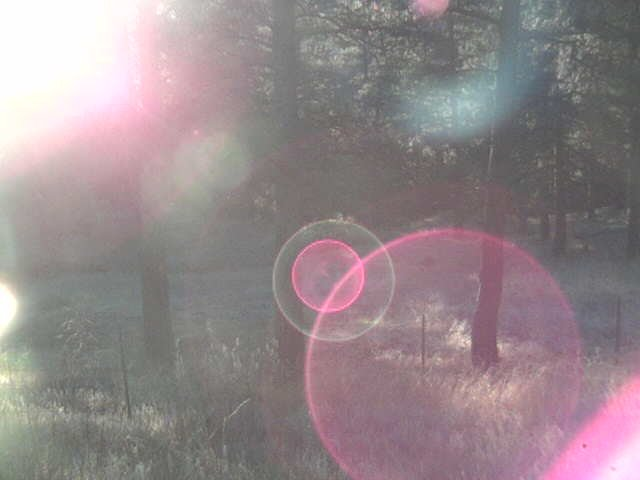
\includegraphics[width=0.45\linewidth, keepaspectratio]{figures/CCTV-Lens-flare.jpg}
}%
\subfigure[Vignetting\newline Image by \cite{image:wikipedia:vignetting}]{
  \label{fig:Vignetting}
  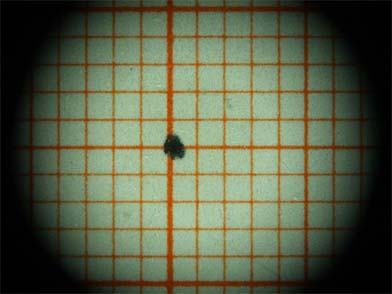
\includegraphics[width=0.45\linewidth, keepaspectratio]{figures/Randabschattung-Mikroskop-Kamera-6.JPG}
}
\subfigure[Smoke\newline Image by \cite{giannarou2013probabilistic}]{
  \label{fig:smoke}
  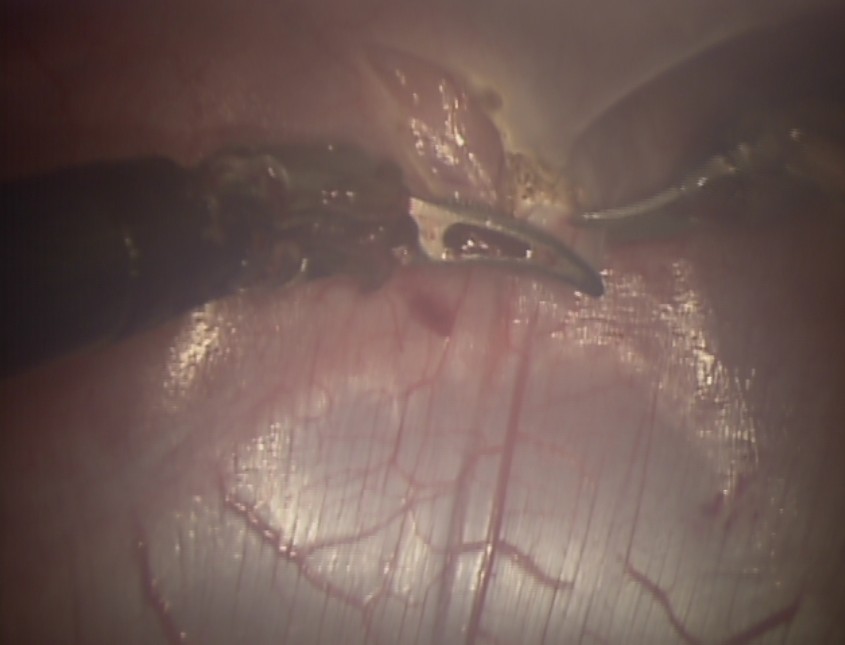
\includegraphics[width=0.45\linewidth, keepaspectratio]{figures/smoke-capture1-033.png}
}%
\subfigure[Camouflage\newline Image by \cite{image:wikipedia:camouflage}]{
  \label{fig:camouflage}
  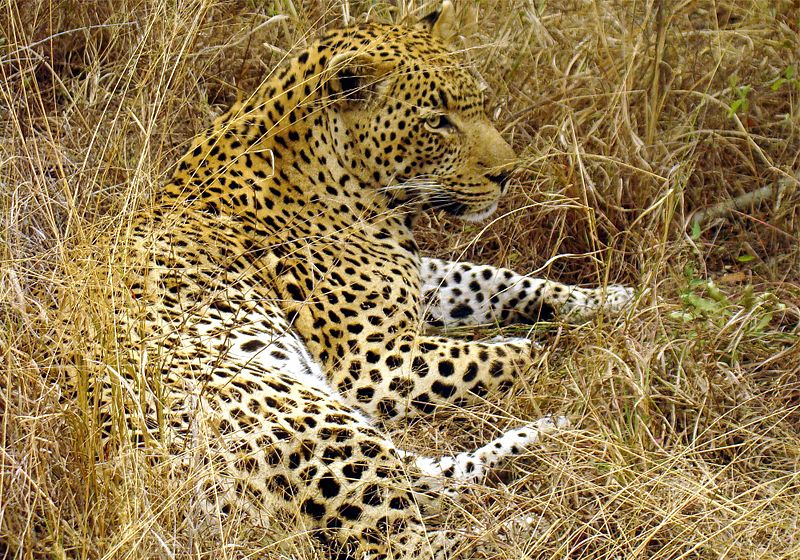
\includegraphics[width=0.45\linewidth, keepaspectratio]{figures/great-male-leopard.JPG}
}
\subfigure[Transparency]{
  \label{fig:transparency-glass}
  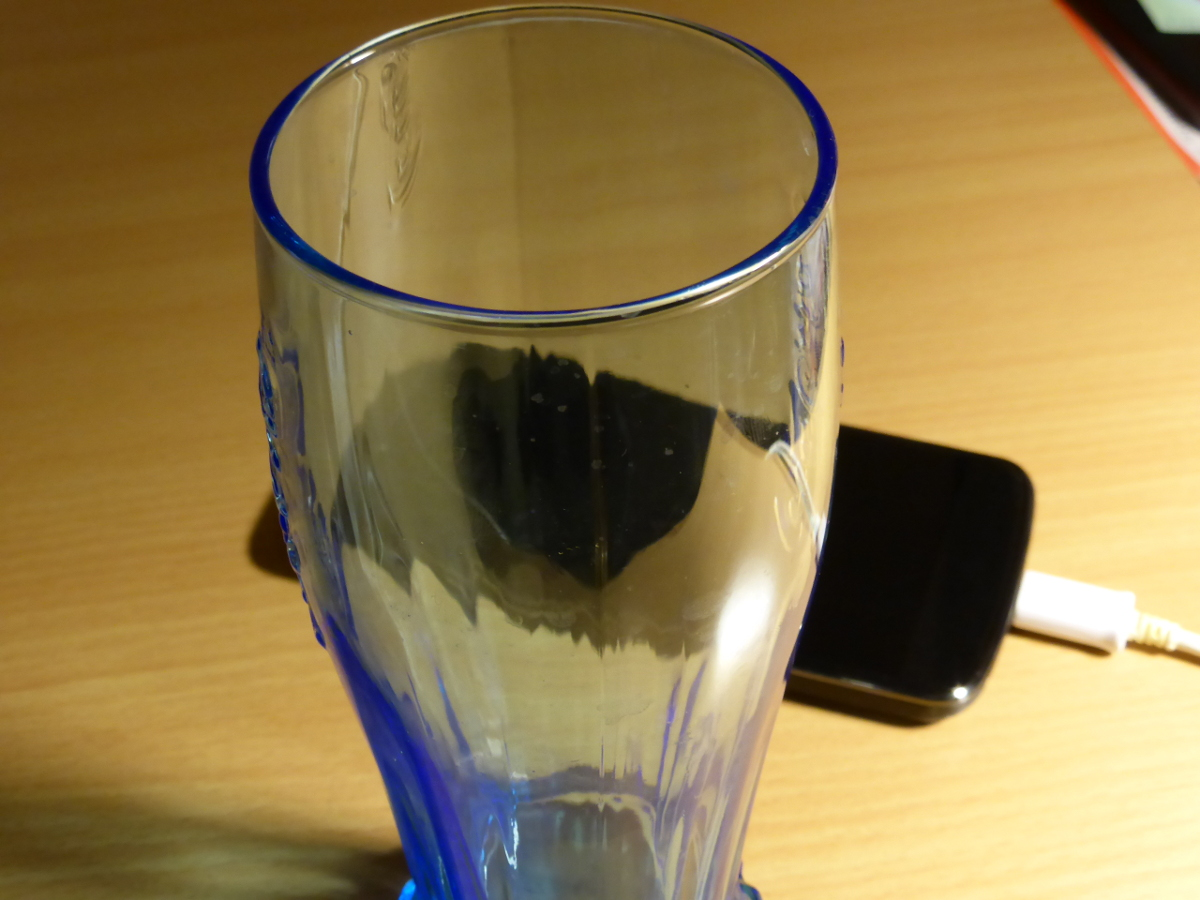
\includegraphics[width=0.45\linewidth, keepaspectratio]{figures/glass-smartphone-table-2.jpg}
}%
\subfigure[Viewpoint]{
  \label{fig:viewpoint}
  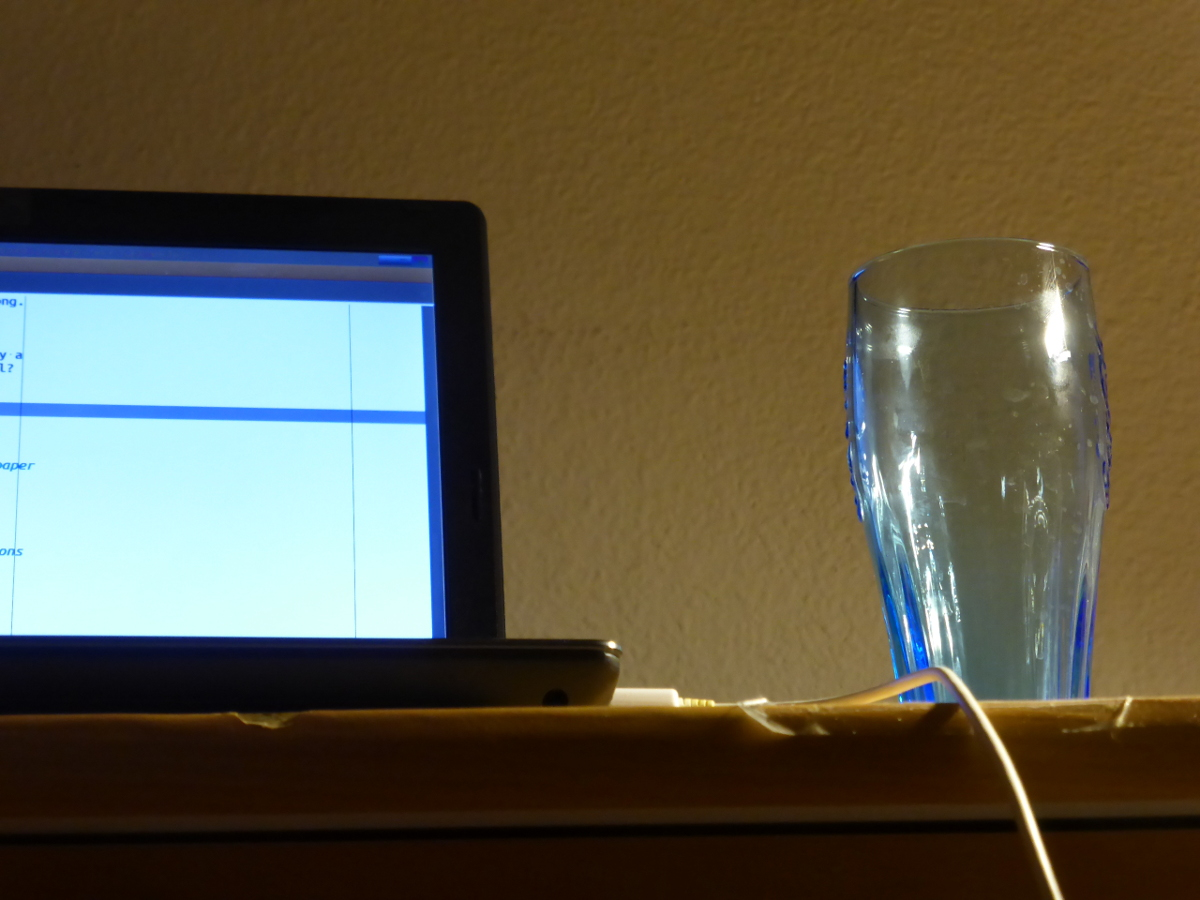
\includegraphics[width=0.45\linewidth, keepaspectratio]{figures/unusual-viewpoint-glass-computer.jpg}
}
\caption{Examples of images which might cause semantic segmentation systems to fail.}
\label{fig:test}
\end{figure}


\subsection{Unsharp images}
Images can be unsharp for a couple of reasons. A problem with the lenses
mechanics, focusing on the wrong point, too quick movement, smoke or foam.
One example of an unsharp image is \cref{fig:smoke}, which was taken during an
in~vivo porcine procedure of diaphragm dissection. The smoke was caused by
cauterization.


\subsection{Other Problems}
If the following effects can occur at all and if they are problems depends
heavily on the problem domain and the used model.

\subsubsection{Partial Occlusions}
Segmentation systems which employ a model of the objects which should be
segmented might suffer from partial occlusions.

\subsubsection{Camouflage}
Some objects, like animals in the wild, actively try to hide
(see~\cref{fig:camouflage} as an example). In other cases it might just be bad
luck that objects are hard for humans to detect. This problem has two
interesting aspects: On the one hand, the segmenting system might suffer from
the same problems as humans do. On the other hand, the segmenting system might
be better than humans are, but it is forced to learn from images labeled by
humans. If the labels are wrong, the system is forced to learn something wrong.

\subsubsection{Semi-transparent Occlusion}
Some objects like drinking glasses can be visible and still leave the object
behind them visible as shown in \cref{fig:transparency-glass}. This is mainly a
definition problem: Is the seen pixel the glass label or the smartphone label?

\subsubsection{Viewpoints}
Changes in viewpoints can be a problem, if they don't occur in the training
data. For example, an image captioning system which was trained on photographs
of professional photographers might not have photos from the point of view of
a child. This is visualized in \cref{fig:viewpoint}.

% \subsubsection{Strong Contrast}
% Strong contrast on the same object, e.g. butterflies or printed pieces of paper
% https://commons.wikimedia.org/wiki/File:Nymphalis_io_Luc_Viatour.jpg


% \begin{itemize}
% %    \item reflections - https://commons.wikimedia.org/wiki/Category:Reflections
%     % https://commons.wikimedia.org/wiki/File:Light_through_glass.jpg
%     % https://commons.wikimedia.org/wiki/Glass
% \end{itemize}

% %!TEX root = vorlage.tex

\section{Speed-ups for Segmentation}

% %!TEX root = vorlage.tex

\section{Image Enhancement}\label{sec:image-enhancement}
Finally, one step to improve the segmentation accuracy is to enhance the
quality of the input image. Removing noise, scaling and contrast enhancements
are some of the actions one might consider to automatically enhance the quality
of the input images.
% http://www.sciencedirect.com/science/article/pii/S0031320301001789

For example, techniques presented in~\cite{Huang-CVPR-2015} can be used to
enhance the quality of the given image.



\newpage
\bibliography{martin}
\bibliographystyle{IEEEtranSA}
\printglossaries%

%!TEX root = vorlage.tex

\clearpage\onecolumn
\begin{appendices}
\section{Tables}
\begin{table}[ht]
    \centering
    \begin{tabular}{llrrcl}
    \toprule
    Database        & Image Resolution (width $\times$ height) & \parbox{1cm}{\centering Number of\\Images}  & \parbox{1cm}{\centering Number of\\Classes}  & Channels & Data source\\\midrule
    Colon Crypt DB  & $(\SIrange{302}{1116}{\pixel}) \times (\SIrange{349}{875}{\pixel})$            & \num{389}  &  2 & 3        & \cite{colon-crypt-segmentation-db}\\
    DIARETDB1       & $\SI{1500}{\pixel} \times \SI{1500}{\pixel}$                                   &  \num{89}  &  4 & 3        & \cite{kalesnykiene2014diaretdb1}\\
    KITTI Road      & $(\SIrange{1226}{1242}{\pixel}) \times (\SIrange{370}{376}{\pixel})$           & \num{289}  &  2 & 3        & \cite{Fritsch2013ITSC}\\
    MSRCv1          & $(\SIrange{213}{320}{\pixel}) \times (\SIrange{213}{320}{\pixel})$             &  \num{240} &  9 & 3        & \cite{MSRC-data}\\
    MSRCv2          & $(\SIrange{213}{320}{\pixel}) \times (\SIrange{162}{320}{\pixel})$             & \num{591}  & 23 & 3        & \cite{MSRC-data}\\
    PASCAL VOC 2012 & $(\SIrange{142}{500}{\pixel}) \times (\hphantom{0}\SIrange{71}{500}{\pixel})$  & \num{2913} & 20 & 3        & \cite{pascal-voc-2012-data}  \\
    Warwick-QU      & $(\SIrange{567}{775}{\pixel}) \times (\SIrange{430}{522}{\pixel})$             & \num{165}  &  5 & 3        & \cite{coelho2009nuclear}\\
    \bottomrule
    \end{tabular}
    \caption{An overview over publicly available image segmentation databases.}
    \label{table:segmentation-databases}
\end{table}
\end{appendices}


\end{document}
